\documentclass{article}
\usepackage{arxiv}

\usepackage[utf8]{inputenc}
\usepackage[english]{babel}
\usepackage[T1]{fontenc}
\usepackage{url}
\usepackage{booktabs}
\usepackage{amsfonts}
\usepackage{nicefrac}
\usepackage{microtype}
\usepackage{lipsum}
\usepackage{graphicx}
\usepackage{natbib}
\usepackage{doi}
\usepackage[dvipsnames]{xcolor}
\usepackage[dvipsnames]{xcolor}
\usepackage{tablefootnote}
\usepackage{amssymb}


\title{Optimizing Computational Graph Configurations for TPU Compilers with GNNs}

\author{ Bessonov A. \\
	M. V. Lomonosov Moscow State University, \\
	the departament of mathematical methods \\ of prediction , 417 group\\
	\texttt{beccohov.a@yandex.ru} \\
	%% examples of more authors
	\And
        Djakonov A. \\
	Phd.         \\
	Central Tinkoff University, Russia \thanks{Science advisor} \\
	\texttt{djakonov@mail.ru} \\
	%% \AND
	%% Coauthor \\
	%% Affiliation \\
	%% Address \\
	%% \texttt{email} \\
	%% \And
	%% Coauthor \\
	%% Affiliation \\
	%% Address \\
	%% \texttt{email} \\
	%% \And
	%% Coauthor \\
	%% Affiliation \\
	%% Address \\
	%% \texttt{email} \\
}
\date{}

\renewcommand{\shorttitle}{\textit{arXiv} Template}

%%% Add PDF metadata to help others organize their library
%%% Once the PDF is generated, you can check the metadata with
%%% $ pdfinfo template.pdf
\hypersetup{
pdftitle={A template for the arxiv style},
pdfsubject={q-bio.NC, q-bio.QM},
pdfauthor={David S.~Hippocampus, Elias D.~Striatum},
pdfkeywords={First keyword, Second keyword, More},
}

\begin{document}
\maketitle

\begin{abstract}
This paper is focused on the challenge of finding optimal compiler configurations for deep learning models, a prominent research area for both engineers and researchers. The importance of hardware performance evaluation models in code optimization is stressed, as it aid compilers in making heuristic decisions and determining the most suitable configuration for various computational programs. Owing to the large-scale nature of computational graphs, consisting of tens of thousands of nodes and edges, conventional analysis methods prove inadequate. An efficient approach is proposed for ranking computational graph configurations, employing graph neural networks, and considering their expected execution time on TPUs. Our method circumvents excessive computational costs and enables training on extensive graphs, making it a highly advantageous contribution to the field.

\end{abstract}


\keywords{TPU XLA \and Compiliers \and AI optimization}
\section{Introduction}
Achieving remarkable performance in a broad range of deep learning applications often hinges on increasing the size of models \cite{kaplan2020scaling}. Nevertheless, the escalation of model parameters introduces numerous challenges, particularly in the realm of training efficiency. Modern Tensor Processing Units (TPUs) and Graphics Processing Units (GPUs) accelerators are sensitive to computational graph configurations (\cite{mangpo2023tpugraphs}, \cite{norrie2020google}, \cite{patterson201850}). Factors such as tensor shapes, transformation orders, and various compiler and operation settings affect the efficiency of an identical computational task \cite{kumar2019scale}.

Deep learning models can be represented as graphs, with nodes signifying tensor operations (e.g., matrix multiplication, convolution, etc.) and edges denoting tensors. The compilation configuration determines how the compiler modifies the graph for a certain optimization pass. In particular, the XLA compiler (\cite{artemev2022memory}) can manage two types of configurations/optimizations, including:

\begin{itemize}
\item Layout configuration - directing the placement of graph tensors in physical memory by establishing dimension order for each operation node's input and output.
\item Tile configuration - controlling the "tile" size of every fused subgraph within the XLA tiling setup.
\end{itemize}

To trial suggested approach, the TpuGraphs dataset \cite{mangpo2023tpugraphs} was employed as primary experimental resource. A primary challenge associated with computational graph exploration resides in their unwieldy dimensions, making standard graph models impractical (Fig. \ref{fig:tpu_dataset} shows specifics of data). Additionally, techniques that address ultra-large graphs prove excessive and yield suboptimal outcomes. On average, layout graphs contain approximately 10,000 to 50,000 nodes, rendering state-of-the-art (SOTA) graph model training use of the full context unfeasible (\cite{rampavsek2022recipe}, \cite{chen2022nagphormer}, \cite{zhang2023large}).

To surmount these limitations, the Graph Segment Training (GST) \cite{cao2023learning} method is used, enabling the aggregation of large graph properties without necessitating training on the entire graph. This novel technique refrains from error backpropagation across the entire graph during the training process, thus offering a more efficient and effective solution for deep learning applications.  It is noticeable that the same problems with extending context are a hot topic in NLP (\cite{dai2019transformer}) as well as in RL (\cite{bessonov2023recurrent}).

\begin{figure}
\label{fig:tpu_dataset}
    \centering
    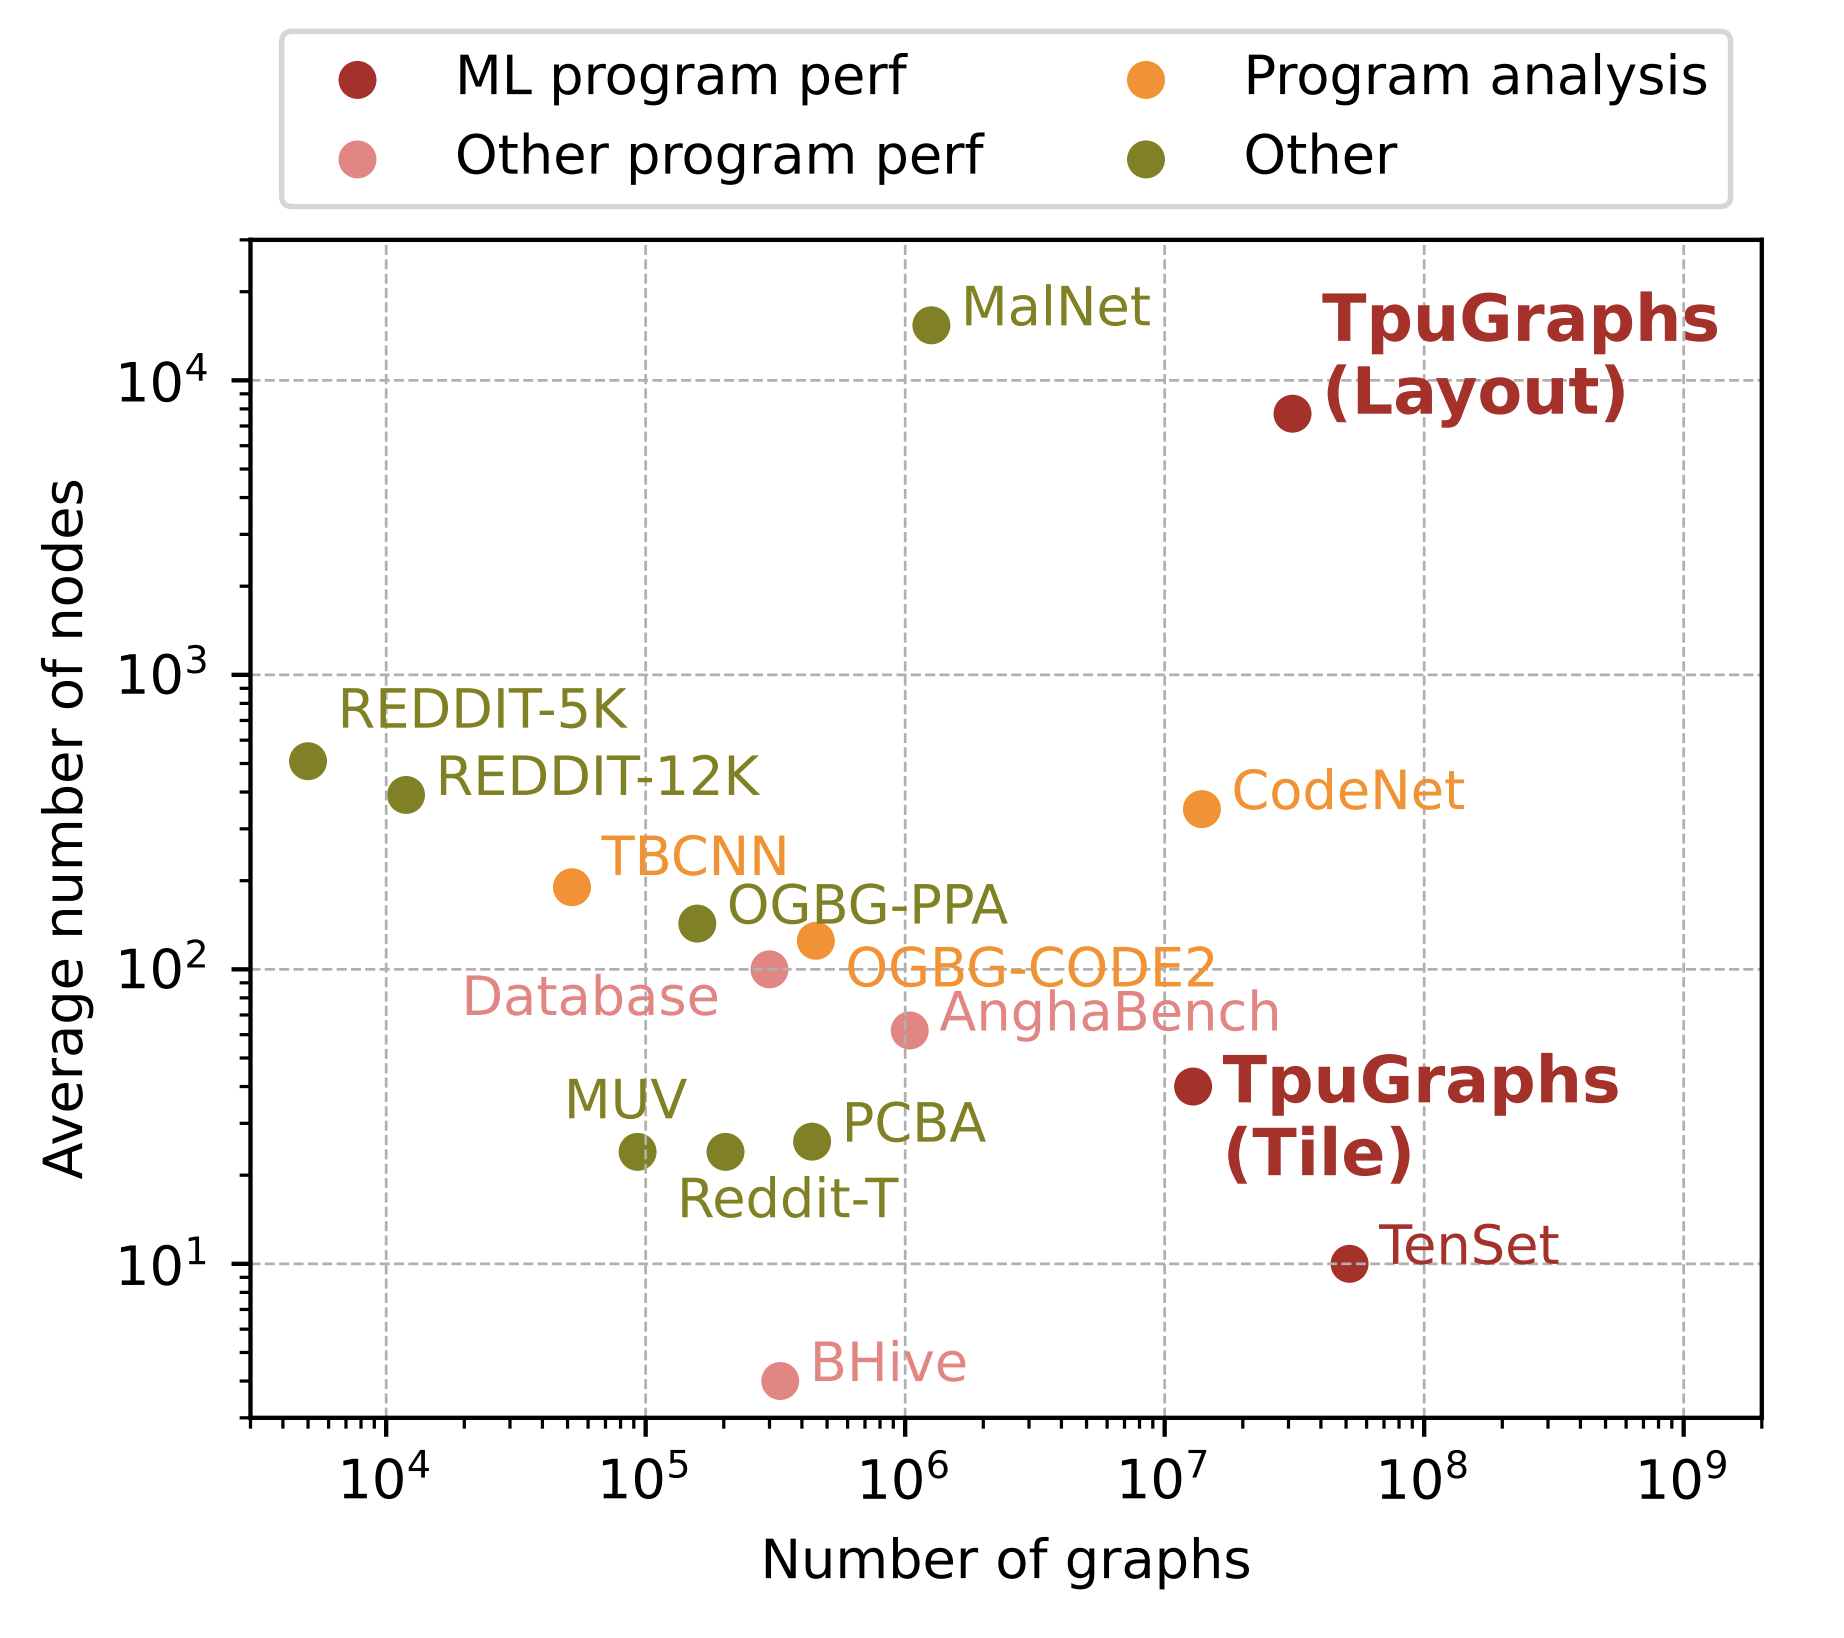
\includegraphics[scale=0.35]{figures/tpu_dataset.png}
    \caption{Scale of TPUGraphs compared to other
graph property prediction datasets.}
\end{figure}



\section{Problem statement}
\label{sec:headings}

The primary task at hand involves obtaining a ranked list of layout configurations for a computational graph's dataset, in accordance with anticipated execution times. To gauge the quality of these rankings, we employ the Kendall rank correlation coefficient as a performance metric, reflecting the extent to which the model-predicted order aligns with the actual order of configurations by execution time.

Popular strategies for seeking optimal configurations, such as genetic algorithms \cite{taugtekin2021foga}, simulated annealing, and Langevin dynamics \cite{garriga2021exact}, necessitate access to a utility function (i.e., the model's prediction). Consequently, it is essential for the model to effectively maintain the configurations' order, ranging from the fastest to the slowest. This fidelity to ordering can be harnessed when searching for optimal configurations in compilers, substantiating the choice to use the Kendall rank correlation coefficient as the most suitable metric for evaluation (see Eq.\ref{eq:tau_coeff} for reference).
\begin{equation}
\label{eq:tau_coeff}
    \tau = \frac{2}{n(n-1)}\sum_{i < j} sgn(x_i - x_j) sgn(y_i - y_j)
\end{equation}
Given the distinct characteristics of the TPU dataset, it comprises two types of graphs (refer to Fig \ref{fig:tpu_graph} for illustration). Each node possesses an operation code, a feature vector, and an optional configuration feature vector specific to layout configurations. The large-scale nature of these graphs demands a training approach that accommodates their enormity. Consequently, we must employ high-quality approximate graph embedding techniques that minimize representation inaccuracies for tractable training, because the majority of large graph models are adopted for extremely large graphs with over many hundreds of thousands nodes \cite{lerer2019pytorch}, \cite{xu2018powerful}.

Addressing this problem, the challenges posed by the TPU dataset and emphasizing the necessity for advanced graph embedding methods that account for large graphs while minimizing losses in precision. This concise yet scientific exposition lays the foundation for the exploration and methodology that will follow in subsequent sections.


\begin{figure}
\label{fig:tpu_graph}
    \centering
    \includegraphics[scale=0.5]{figures/tpu_graph_examples.png}
    \caption{A node represents a tensor operator, annotated with its output tensor shape $[n0, n1, ...]$,
where $n_i$
is the size of dimension i. Layout $\{d0, d1, ...\}$ represents minor-to-major ordering in
memory. Applied configurations are highlighted in \textcolor{red}{red}, and other valid configurations are highlighted
in \textcolor{SkyBlue}{blue}. A layout configuration specifies the layouts of inputs and outputs of influential operators (i.e.,
convolution and reshape). A copy operator is inserted when there is a layout mismatch.}
\end{figure}

\section{Approach}
\label{sec:approach}

To tackle the aforementioned challenges, Graph Segment Training (GST) was employed as illustrated in Fig. \ref{fig:main_schema}. This method involves dividing each large graph into smaller, controlled-size segments during the preprocessing phase. Throughout the training process, a random subset of segments at each step is selected, updating the model without utilizing the entire graph, i.e. $$\mathcal{G}^{(i)} = \bigoplus \mathcal{G}^{(i)}_{j}, \; \; \; \; \; j \in \mathcal{J} = \{1, ... , \frac{\mathcal{L}(\mathcal{G}^{(i)})}{\mathcal{K}}\}$$, where $\mathcal{K}$ is maximum allowed subgraph nodes count and $\mathcal{L}(\mathcal{G}^{(i)})$ is a count of nodes in graph $\mathcal{G}^{(i)}$ (see \cite{cao2023learning} for more details). 

Consequently, intermediate activations must only be maintained for a few segments during backpropagation, while embeddings for the remaining segments are generated without preserving intermediate activations:
$$\bigoplus \mathcal{G}^{(i)}_{j} = (\bigoplus_{k \in \mathcal{Y}} \mathcal{G}^{(i)}_{k}) + (\bigoplus_{m \in \mathcal{M}} \mathcal{G}^{(i)}_{m}), \; \; \; \; \;j \in \mathcal{J} = \{1, ... , \frac{\mathcal{L}(\mathcal{G}^{(i)})}{\mathcal{K}}\}, $$

$$\mathcal{Y} \cup \mathcal{M} = \mathcal{J}, \:\:\:\;\: \mathcal{Y}  \cap \mathcal{M} = \varnothing $$
By subsequently merging all segment embeddings, we produce an embedding for the original large graph, facilitating prediction.

The approach ensures that each large graph adheres to an upper bound on memory consumption during training, regardless of its initial size. Consequently, this method enables training on large graphs without encountering out-of-memory (OOM) issues, even when computational resources are limited.

To further enhance the efficiency of the training process, a historical embedding table is incorporated, streamlining the generation of graph segment embeddings that do not necessitate gradients. By leveraging historical embeddings, we bypass superfluous computation on these segments.

Each $\mathcal{G}^{(i)}_{j}$ embedding is a result of applying three type of encoders, as shown in \ref{fig:main_schema}, i.e.:
$$
\mathcal{G}^{(i)}_{j} = \mathcal{M}_1(opcodes) + \mathcal{M}_2(configs) + \mathcal{M}_3(nodes),
$$
where $\mathcal{M}_i$ is appropriate embedder (linear layer without bias in this case).

Notably, topological sorting of nodes in the dataset allows for more effective segmentation by taking contiguous subsequences of nodes.

\begin{figure}
\label{fig:main_schema}
    \centering
    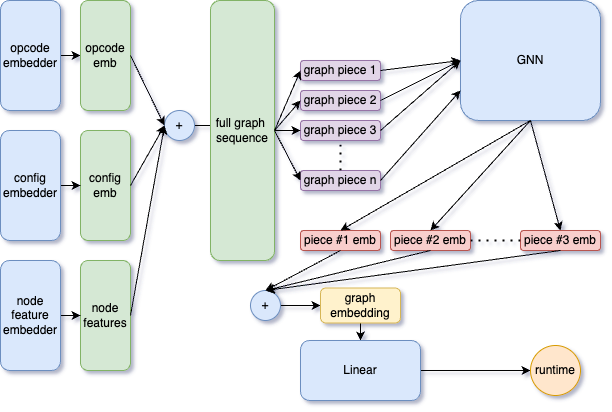
\includegraphics[scale=0.6]{figures/main_schema.png}
    \caption{Used GST approach for segment training. Red arrows show the gradient flow during the backward propagation. For each feature type used separate embedder.}
\end{figure}
\section{Experiments}

To evaluate Graph Segment Training (GST) approach, two common baseline models were implemented for comparison. The first baseline, referred to as the \textit{Pooling Model}, employs a linear layer over the mean-pooled configuration features and node features across the entire graph.

The second approach, similar to GST, does not include graph feature sequence partitioning. Instead, it selects a random contiguous subsequence of nodes, and prior to backpropagation, halts gradients from all other nodes (see Fig. \ref{fig:baseline_scheme}). This model is designated as \textit{Partitioning}. Additionally, we applied the Graph Attention Network (GAT, \cite{velivckovic2017graph}) to this problem for further comparison.

The comparative results can be found in Tab. \ref{tab:table}. As evidenced by the experimental data, the GST approach maintains reasonable quality while enabling training on large graphs. Applying GAT directly without the GST method results in memory limitations. Simultaneously, the \textit{Partitioning} training demonstrates reduced performance despite employing the same GAT model, underscoring the significance of the GST method to model performance. Moreover, GST preserves a quality comparable to the GAT model trained on a full graph for moderate graphs, showcasing the strong graph representation learning capability when dealing with large graphs.

\begin{table}
	\caption{Comparisson of different methods across the graphs}
	\centering
	\begin{tabular}{llllll}
		\toprule
		\multicolumn{5}{c}{TPU graph type}                   \\
		\cmidrule(r){1-5}
		Tile XLA \tablefootnote{Here used another metric written as $Q = 2 - \frac{min_{i \in K} y_{pred}}{min_{i \in A} y}$, where $K$ = 5 - top predicted configurations actual runtimes, A - real top configurations}     &  Layout nlp random     &  Layout nlp default     & Layout xla random & Layout xla default     & Method \\
		\midrule
		0.85     &  0.82 &  0.42     & 0.26 & 0.11  & GST     \\
		0.45     &  0.32   &  0.12  & 0.11     & 0.05 & Pooling Model      \\
		0.67     &  0.62  &  0.27   & 0.21     & 0.12       & Partitioning  \\
            0.92     &  OOM   &  OOM  & OOM     & OOM & GAT      \\
		\bottomrule
	\end{tabular}
	\label{tab:table}
\end{table}
\begin{figure}
\label{fig:baseline_scheme}
    \centering
    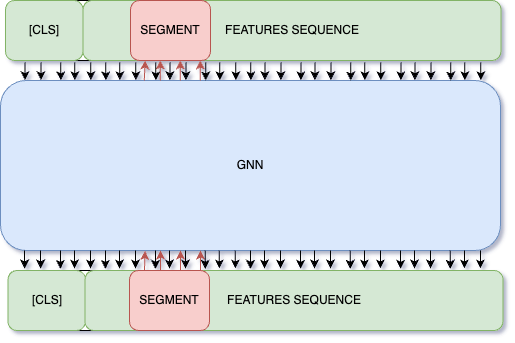
\includegraphics[scale=0.5]{figures/baseline_scheme.png}
    \caption{Baseline with graph backward partition. The only subsequence of nodes embeddings chosen to make a backward pass. Forward pass flow shown as black arrows, red arrows show backward pass path.}
\end{figure}

\section{Conclusion}
In this study, a solution to alleviate the challenges associated with large graph representation is presented in the context of TPU compiler optimization. Proposed method, Graph Segment Training (GST), enables efficient training on large graphs while consuming significantly less GPU/TPU memory, delivering quality comparable to full graph training.

As this research is ongoing, it is planned to implement further improvements to enhance the GST framework. It is anticipated that the findings and advancements presented in this paper will contribute to more efficient AI training and evaluation processes. This may ultimately lead to a reduced carbon footprint and facilitate the development of larger models capable of achieving new state-of-the-art results.

\newpage
\bibliographystyle{unsrtnat}
\bibliography{references}

\end{document}
